\chapter{Introdução}
\label{cap-introducao}

\section{Contexto}
\label{section:contexto}

\citeonline{indiceglobaldoempreendedorismo} afirma que menos de 1\% das empresas do Brasil conseguem manter uma taxa de crescimento acima dos 20\% anuais por um período de três anos consecutivos mas as mesmas foram responsáveis por mais de 40\% dos novos empregos gerados no país, em média elas geram cerca de 100x mais empregos do que as empresas do Brasil. Algumas dessas empresas com alto potencial de crescimento são conhecidas como startups.

\citeonline{Graham2012} diz que o único fator essencial para que uma organização seja classificada como startup é o seu crescimento, para ele qualquer outro fator nada mais é do que um reflexo deste, como uma captação bem sucedida de investimentos. Idealmente Graham defende que elas precisam crescer entre 5 e 7\% por semana e que qualquer indicador acima de 10\% seria algo excepcional.

Para \citeonline{Sutton2000} a característica mais básica de uma startup é ser nova e inexperiente quando comparada com organizações estabelecidas e maduras. Ele também as caracteriza como organizações que trabalham com poucos recursos e geralmente acompanham novas tendências de tecnologia e mercado, além de altamente sensíveis à diversos influenciadores (investidores, clientes, parceiros e concorrentes).

Segundo \citeonline{Ries2011} uma startup é uma instituição humana projetada para criar novos produtos e serviços sob condições de extrema incerteza. Para ele, o maior objetivo de uma startup é descobrir qual o produto certo que os consumidores queiram e estejam dispostos a comprar, e/ou usar, o mais rápido possível.

\citeonline{Paternoster2014} diz que para construir produtos tecnologicamente inovadores geralmente elas precisam utilizar novas tecnologias, ferramentas e técnicas de gestão e desenvolvimento. Esse cenário condiz com o mapeamento realizado por \citeonline{Polovets2014} o qual constatou que a maior parte das startups analisadas utilizam tecnologias modernas como Javascript, Node.js, Ruby, Ruby on Rails, Python e HTML5 e hospedam seus softwares em grandes infraestruturas escaláveis como Amazon Web Services e Heroku. Para \citeonline{isenberg2016} a maior parte das pessoas associa o termo ``startup'' com empresas como o ``Snapchat'' ou o ``WhatsApp''.

De volta ao Brasil, \citeonline{Brinded2015} relata que o país é o terceiro com o maior número de empreendedores do mundo, correspondendo a cerca de 13,8\% da população, como indicado pela Tabela \ref{table:ranking_de_paises_com_mais_empreendedores}. Para \citeonline{Acs2016} um dos destaques do Brasil é a Percepção de Oportunidade\citeonline{schwab2015}, como explicitado pela Figura \ref{figure:gedi_brazil}.

\begin{figure}[!htb]
	\centering
	\includegraphics[width=11cm,angle=0]{figuras/gedi_brazil}
	\caption{Comparação dos pilares brasileiros de acordo com o Índice Global de Empreendedorismo}
	\label{figure:gedi_brazil}
\end{figure}

Governos das três esferas brasileiras (Federal, Estaduais e Municipais) estão em busca de formas para atrair investimentos externos, gerar de empregos e aumentar a arrecadação de impostos por meio de apoio aos seus ecossistemas empreendedores de tecnologia com de iniciativas de fomento e capacitação como o Startup Brasil, Inovativa Brasil, Sebrae de Inovacão, Fundo Criatec, editais de subvenção por meio de Fundações de Apoio à Pesquisa, FINEP, etc. Além disso alguns projetos de lei como a Lei da Inovação e o Marco Legal da Ciência, Tecnologia e Inovação buscam trazer flexibilidade para o ambiente regulatório do Brasil com o objetivo de aumentar as chances de sucesso e crescimento das startups.

Trazendo para o contexto de Brasília, a cidade vive um dos seus melhores momentos para o crescimento do ecossistema de startups local, embora o país e a cidade estejam passando por uma recessão e crises política e econômica o cenário nunca foi tão favorável e como reflexo é vísivel que o interesse dos brasilienses tem aumentado, a capital também demonstrou seu potencial com a atração de grandes eventos como o AgileBrazil, a World Conference on International Telecommunications, a Campus Party e diversos outros menores organizados pela comunidade local, como meetups e a Capital Empreendedora. \citeonline{Sun2011} relata que a Professora da Harvard Business School Janet. J. Kraus acredita que as crises são os melhores momentos para se iniciar um novo negócio, justamente quando os custos de oportunidade são baixos. Ela defende que se o empreendedor é capaz de lucrar durante uma crise então o negócio será ainda mais lucrativo quando o mercado se recuperar.

A baixa expectativa de concursos públicos para os próximos anostambém é um fator favorável para o empreendedorismo, forçando os jovens a buscar alternativas que não a estabilidade financeira provida pelo serviço público, principal motivo para uma Cultura Empreendedora tão ruim na cidade, como constatado pela \citeonline{indiceglobaldoempreendedorismo}, embora Brasília se destaque no que tange o Mercado e Acesso à Capital. 

\section{Justificativa}
\label{section:justificativa}

\citeonline{Paternoster2014} enfatiza que pesquisas acadêmicas são necessárias para apoiar as atividades relacionadas a startups e guiar as ações de diversos atores que compõem um ecossistema, como empreendedores, agentes públicos, investidores e acadêmicos.

Com base em uma análise das principais publicações acerca do tema nos últimos 300 anos \citeonline{Filion1998} divide o progresso dos estudos acerca do empreendedorismo em cinco períodos representados pela Tabela \ref{table:tendencias_nas_publicacoes_acerca_do_empreendedorismo}.

\begin{table}[!htb]
	\centering
	\begin{tabular}{ | p{6cm} | p{6cm} | p{3cm} | }
		\hline
		Tema & Perspectiva & Período \\ \hline
		O que fazem os empreendedores & Econômica & 1700 - 1950 \\ \hline
		Quem são os empreendedores & Comportamental & 1960 - 1980 \\ \hline
		O que fazem os empreendedores & Administrativa(finanças, marketing, operações, recursos humanos) & 1980 - Atual \\ \hline
		Quais tipos de suporte são necessários para empreendedores & Ciências Sociais(incluindo economia, geográfia e sociologia) & 1985 - Atual \\ \hline
		O que são atividades empreendedoras e quais Competências são necessárias & Empreendedorismo & 1990 - Atual \\ \hline
	\end{tabular}
	\caption{Tendências nas publicações acerca do Empreendedorismo por \cite{Filion1998}}
	\label{table:tendencias_nas_publicacoes_acerca_do_empreendedorismo}
\end{table}


Embora \citeonline{Filion1998} tenha relatado a época que pouco se explorou sobre ecossistemas e como os mesmos contribuem para o desenvolvimento local \citeonline{Cukier2016} conseguiu demonstrar que nos últimos sete anos houve um crescimento superior a 1000\% na quantidade de artigos acadêmicos com o termo ``Startup Ecosystems'' indexados pelo Google Scholar. \citeonline{Spigel2015} diz que o estudo de ecossistemas empreendedores se tornaram uma ferramenta popular para o estudo do empreendedorismo de alto crescimento sob o ponto de vista geográfico, \citeonline{Unterkalmsteiner2016} relatam que as quatro grandes perguntas de pesquisa sobre o estudo de ecossistemas de startups de tecnologia que precisam ser respondidas envolvem os elementos chaves de um ecossistema frutífero, os tipos de ecossistemas (diferentes tamanhos, setores da tecnologia, etc), como eles evoluem com o passar do tempo e como mensurar a qualidade de um determinado ecossistema de startups. 

\
\begin{figure}[!htb]
	\centering
	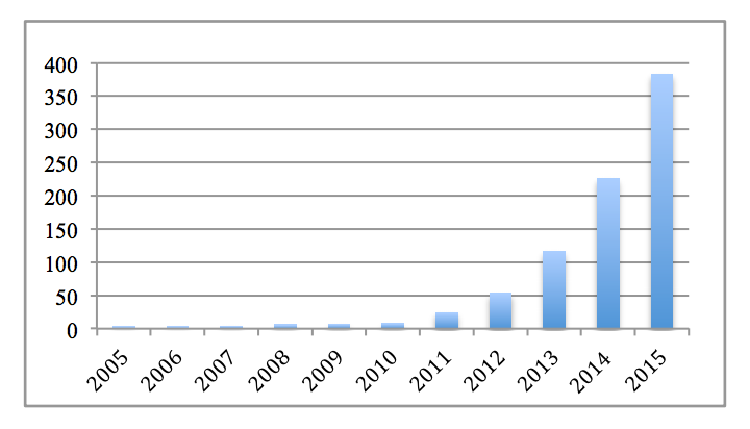
\includegraphics[width=11cm,angle=0]{figuras/papers_about_startup_ecosystems}
	\caption{Quantidade de papers com o termo ``Startup Ecosystem'' por \citeonline{Cukier2016}}
	\label{figure:papers_about_startup_ecosystems}
\end{figure}

Portanto, nota-se que é crescente a busca acerca do que tange o mundo das startups e como ecossistemas são compostos por elementos importantes para o seu crescimento. O objetivo deste estudo é produzir um relatório a respeito do ecossistema de startups de tecnologia de Brasília que possa ser de utilidade de gestores públicos, empreendedores e sociedade civil interessada.

\section{Questão de Pesquisa}
\label{section:questao_de_pesquisa}

Qual o atual momento e o grau de maturidade do Ecossistema de Startups de Tecnologia do Distrito Federal?

\section{Objetivo Geral}
\label{section:objetivo_geral}

Aplicar a metodologia de avaliação de ecossistemas de startups de tecnologia criada por \citeonline{Kon2014} no contexto do Distrito Federal.

\section{Objetivos Específicos}
\label{section:objetivos_especificos}

Este trabalho consiste em um estudo de caráter exploratório do ecossistema de startups de tecnologia do Distrito Federal com o objetivo específico de conhecê-lo para que seja feita uma avaliação do seu atual momento e sua maturidade. Como resultado final é esperado uma síntese dos dados coletados de forma a permitir comparações com outros ecossistemas avaliados com a mesma metodologia e uma visão generalista de algumas das características como pontos fortes e pontos de melhora do ecossistema local de acordo com a visão dos atores que o compõem. 

\section{Organização do Trabalho}
\label{section:organizacao_do_trabalho}

Este Trabalho de Conclusão de Curso em mãos está organizado em quatro capítulos: primeiramente uma breve introdução com o contexto o qual está inserido e os objetivos de pesquisa.

O segundo capítulo explora o cenário de pesquisa em torno de ecossistemas de startups e descreve a metodologia que será aplicada em Brasília, principalmente no que tange os indicadores utilizados para mensurar sua maturidade.

O terceiro capítulo apresenta os resultados obtidos, o que fora descoberto, qual a visão dos empreendedores entrevistados e quais ações podem ser tomadas para que o ecossistema do Distrito Federal evolua.

No quarto capítulo é feito um apanhado de tudo o que foi explorado nos capítulos anteriores e o que fora aprendido com o desenvolvimento deste trabalho. Por fim, são apresentados os Anexos e Apêndices mencionados.
